\documentclass[journal,twoside]{JoPhA}

\usepackage{color}
\usepackage{flushend}

\usepackage{fancyvrb}


\usepackage[pdftex]{graphicx}
% declare the path(s) where your graphic files are
\graphicspath{{figures/}}
% and their extensions so you won't have to specify these with
% every instance of \includegraphics
\DeclareGraphicsExtensions{.pdf,.jpeg,.png}

\begin{document}

\title{Cybersecurity in Autonomous Systems: Evaluating the performance of hardened ROS}

\author{David Ma\~nanes, Francisco Javier Rodr\'iguez Lera, Jes\'us Balsa and Vicente Matell\'an,
\IEEEcompsocitemizethanks{
All authors are with the Robotics Group (http://robotica.unileon.es) and the Research Institute on Applied Sciences to Cybersecurity (http://riasc.unileon.es) at Universidad de Le\'on (Spain).

\IEEEcompsocthanksitem Corresponding author: vicente.matellan@unileon.es} % <-this % s
}


\markboth{Workshop on Physical Agents, M\'alaga 2016}%
{Matell\'an et al: Cybersecurity in ROS}
\maketitle


\begin{abstract}
As robotic systems spread, cybersecurity emerges as major concern. Currently most research autonomous systems are built using the ROS framework, along with other commercial software. ROS is a distributed framework where nodes publish information that other nodes consume. This model simplifies data communication but poses a major threat because a malicious process could easily interfere the communications, read private messages or even supersede nodes. In this paper we propose that ROS communications should be ciphered. We also measure how this ciphering affects its performance. We have used three different ciphering techniques: DES, AES and RSA. We have evaluated the performance of the system, both from the computing and the communications points of view. Preliminary results show that symmetric ciphers using private keys impose significant delays.

\end{abstract}


\begin{IEEEkeywords}
autonomous systems, cybersecurity, robotics, performance, cyber-physical systems, ciphers
\end{IEEEkeywords}


\section{Introduction}

\IEEEPARstart{A}{utonomous} systems are spreading not just in the virtual world (Internet, software systems), or in science-fiction movies, but in our ordinary real world. Currently we can find driverless cars in the streets, autonomous vacuum cleaners in our homes, museum guides, hotel assistants, etc. These cyber-physical systems, as any computer-based system, can suffer different types of vulnerabilities, and the need of cybersecurity \cite{Morante2015} is required. 

ROS (Robotic Operating System) \cite{ROS09} has become the most popular framework for developing robotic applications. It started in the research environment, but currently most of manufacturers of commercial platforms use ROS as the {\em de facto} standard for building robotic software. For example, object-manipulation robots like Baxter (by Rethink robotics){\textcolor{red}{[poner REF]}} or service robots as our RB1 (by Robotnik){\textcolor{red}{[poner REF]}} are ROS based platforms.

Our research group is developing assistant robot~\cite{Martin2014} for the elderly. When we initiated experiments involving potential users, caregivers have asked us about the security of our robot, and about the privacy of its communications \cite{Denning2009}. If an assistant robot carrying a camera is deployed in a home, the access to the camera should be secured. Even more when the robot is managing medical information. We have developed all our software for the autonomous behaviour of the robots using ROS, so we need to consider its security.


\subsection{ROS security assestment}

ROS provides specific libraries for robotics as well as classical operating system services such as hardware abstraction (for sensors and actuators), low-level device control, and inter-process communication. Inter-process communication is based on a graph architecture where computation takes place in ROS processes named nodes. These nodes can receive and send messages, but no security was considered in its design. 

ROS framework is basically a message-passing distributed system. Its architecture is based on processes that publish {\em messages} to {\em topics}. For instance, a process ({\em node}) can be in charge of accessing a sensor, making the basic processing of the information, and publishing it as a structure information on a named topic. Another process can {\em subscribe} to this topic, that is, it can read that information, make a decision about the movement of the robot. These commands will be sent to the motors in another topic. These nodes can be running in the same computer or in different computers. 

This approach is very convenient for developers but it is very easily tampered by malicious hackers. For instance in \cite{McClean2013} an experiment involving a ROS-based honeypot is described. The honeypot was a radio model truck with two cameras and a compass as sensors and controlled from a remote ROS node written in Javascript and hosted in a remote enterprise grade web server. Vulnerabilities described in the paper range from plain-text communications, unprotected TCP ports to unencrypted data storage.

These vulnerabilities are a subset of the security problems threatening any computing system:
{\textcolor{red}{No s\'e si merece la pena, demasiado generalista. Igual es mejor hablar más de cosas específicas de robótica y de ROS en particular}}
\begin{enumerate}
 \item Availability: Interruption
 \item Confidenciatily: Interception
 \item Integrity: Modification
 \item Authenticity :Fabrication
\end{enumerate}

Figure \ref{fig:Conceptualmodel} graphically summarizes these problems in our robot.

\begin{figure}[ht]
    \centering
    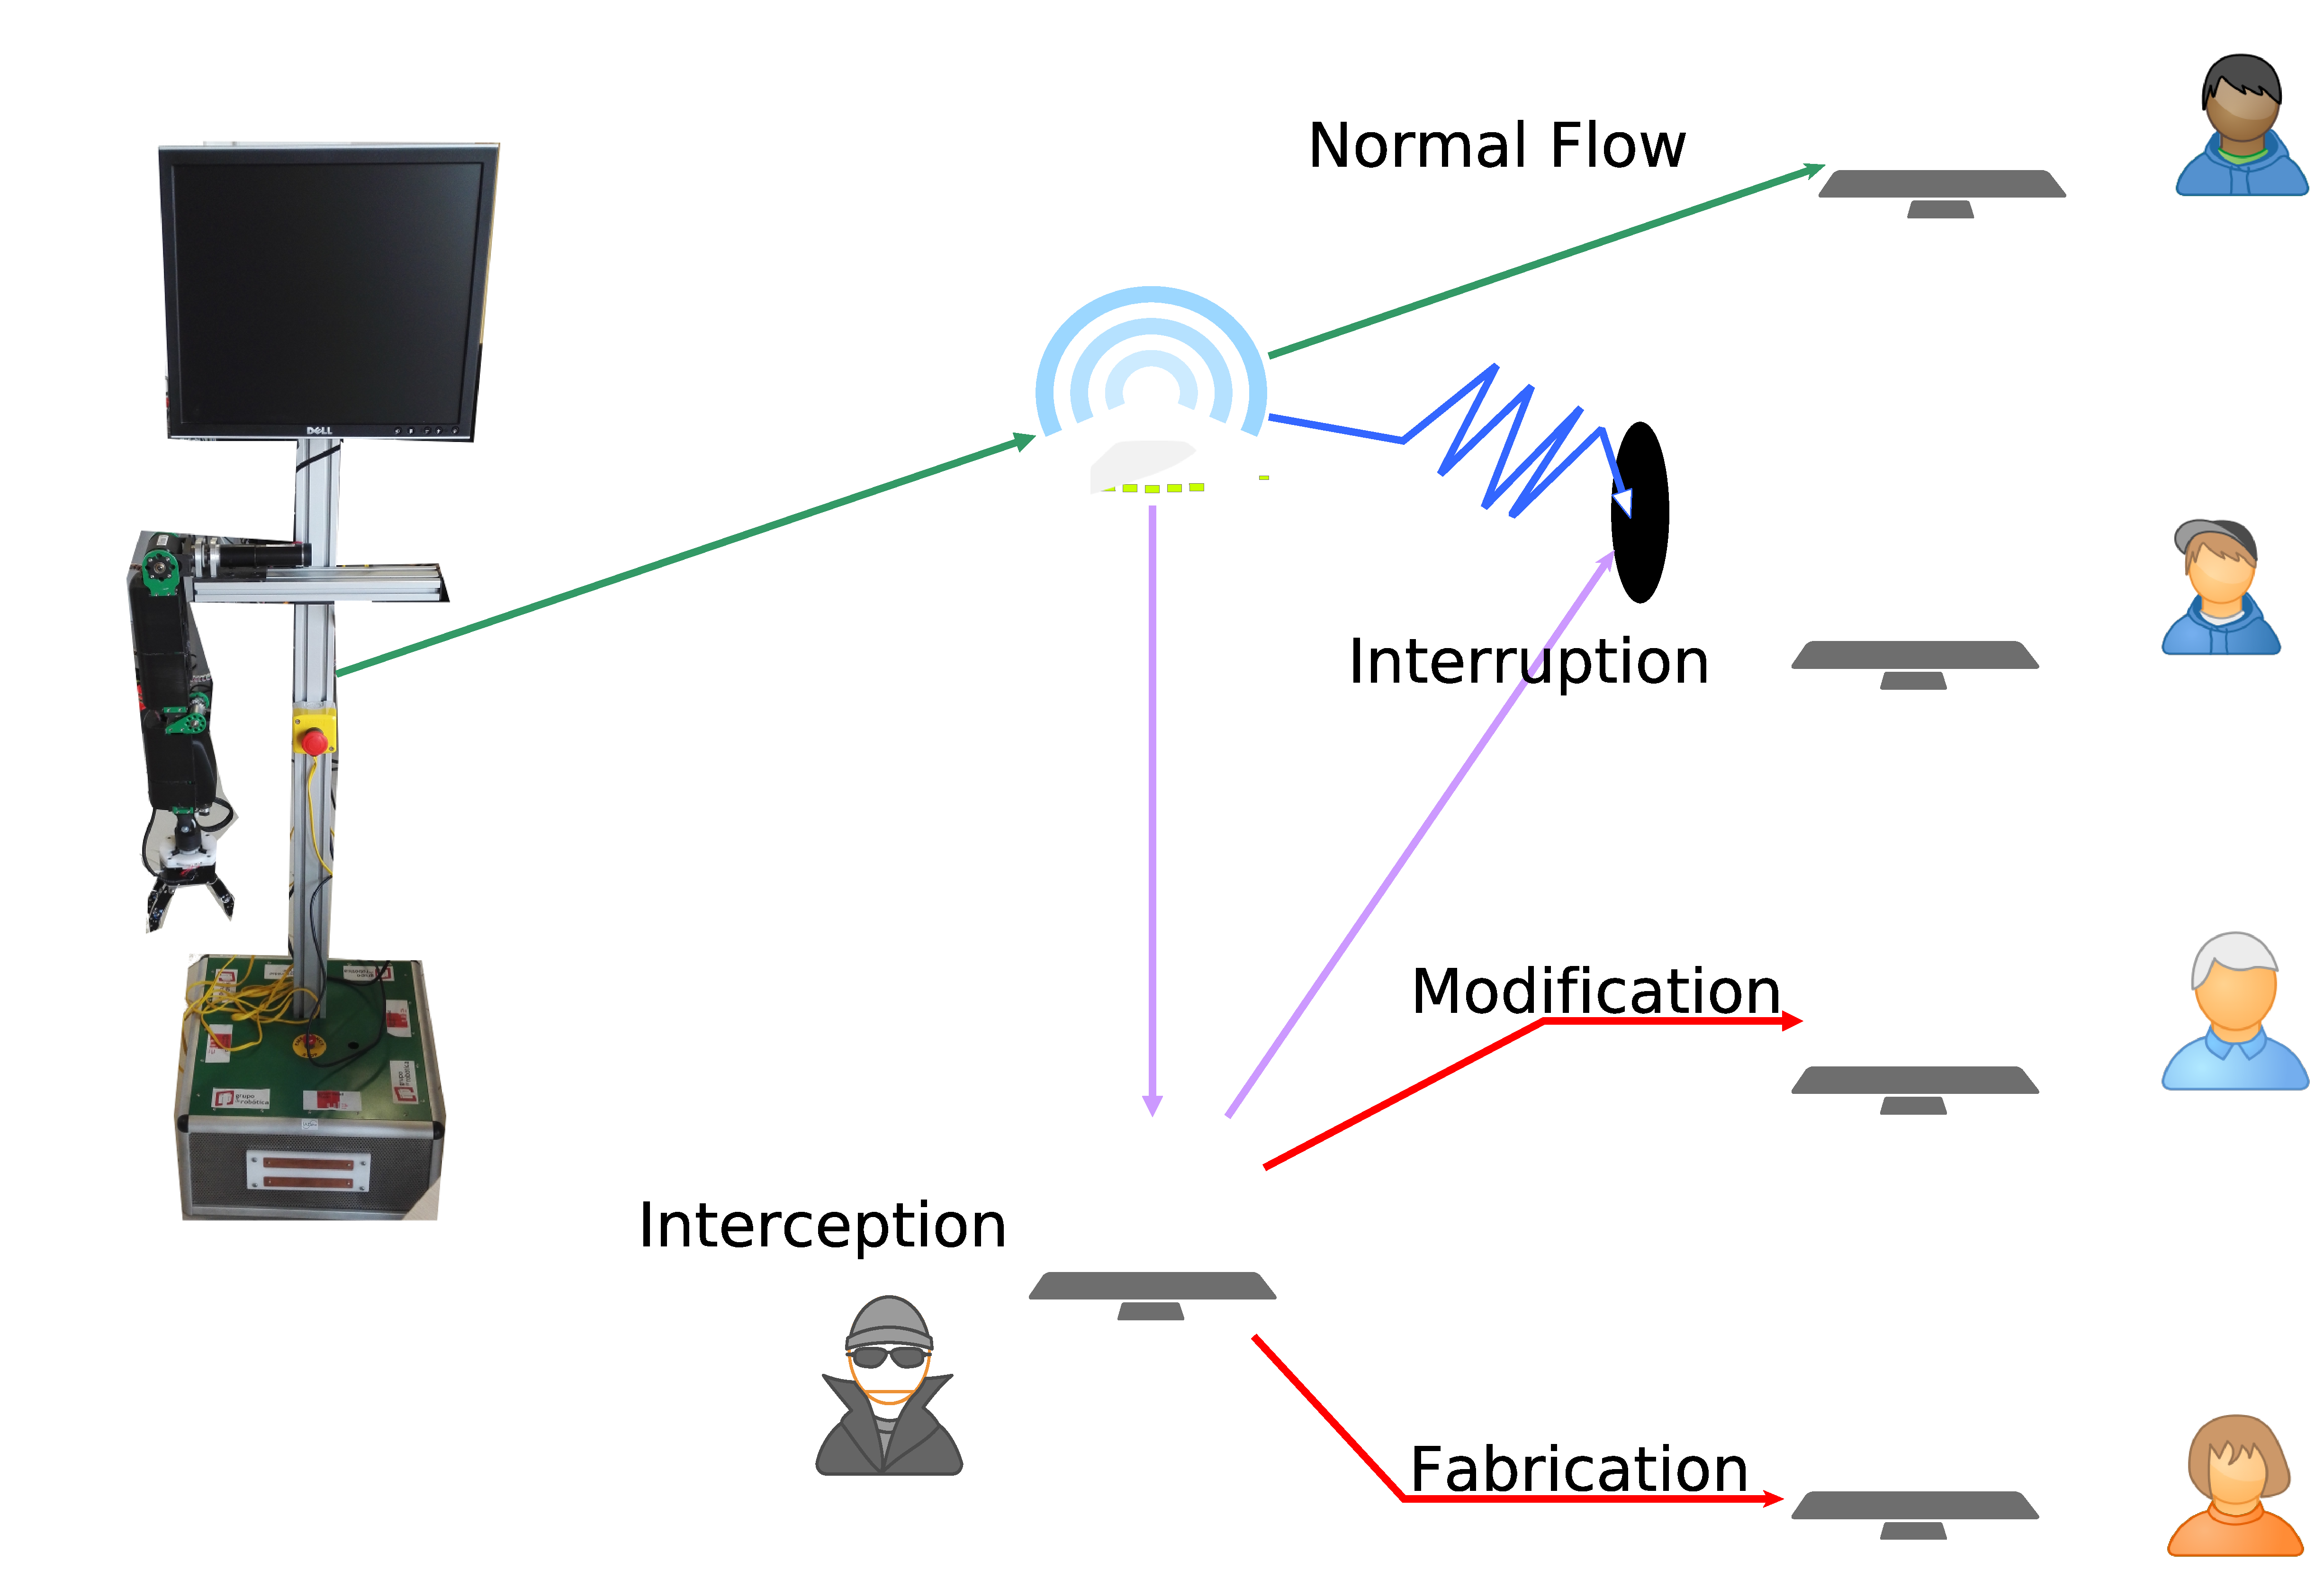
\includegraphics[width=.5\textwidth]{SecurityAttacks.pdf}
    \caption{Conceptual model of the security attacks.}
  \label{fig:Conceptualmodel}
\end{figure}

The first step to solve some of these problems is to secure the communication channels by using a ciphering mechanism. but, how does this systems impact on the performance of a robotic system? This is the goal of this paper, characterize and evaluate different alternatives to secure ROS communication mechanism.

Next section describes the testbed we have designed to measure the performance of the encrypted ROS system. Third section evaluates the data obtained in the experiments and in the last section some conclusions and further work are presented.



\section{Testbed description}

Conventional ROS environment is composed by at least one ROS Master and any laptop clients. The ROS Master is the key element in a ROS environment, it runs as a nameservice.
It also stores topics and services registration information for ROS nodes. 

When a node want to stablish a connection with a topic, it communicate with the Master to advise its registration information. After this step, the node gets more information about other registeres nodes and can stablish new connections approapiately. The Master is updated in real time about clients information, and at the same time callbacks to those related nodes.



% Nodes communicate with the Master to report their registration information. 
% As these nodes communicate with the Master, they can receive information about other registered nodes and make connections as appropriate. The Master will also make callbacks to these nodes when this registration information changes, which allows nodes to dynamically create connections as new nodes are run. 

Figure~\ref{fig:TestBed} provides the graphical representation of this situation. In this case, two clients are connected to a topic. It is transparent to ROS Master this situation,  
The standard process starts with a basic sensor node (BSN). We have defined as BSN those ROS nodes in charge of to publish the information from the sensor.



We have prepared a  testbed with two laptopts 

% \subsection{Simulated testedbed}

We have installed ROS Jade in two computers connected through a wired Ethernet 10/100 switch (model XXXX). In the first computer we have connected a Xtion camera and a Hokuyo laser. In the second computer have run a node visualizing the information from the sensors. Figure \ref{fig:maqueta} shows this environment.


% Then we modified the standard ROS implementation. We changed the TCP/IP sockets based implementation by ciphered ones.

In this first approach we have changed the info published by the node, and instead of publish the information in a clean way, we publish the information encrypted.
We use the DES3 algorithm that provides a 
Triple DES references the Triple Data Encryption Algorithm (3DES or TDEA or Triple DEA). It is a symmetric-key block cipher and from a high level point of view the algoritm applies the Data Encryption Standard (DES) cipher algorithm three times to each data block. It is standarized by NIST (Recommendation for
the Triple Data Encryption Algorithm (TDEA) Block Cipher) NIST Special Publication 800-67.

It has a fixed data block size of 8 bytes. Its keys are 128 (Option 1) or 192 bits (Option 2) long. However, 1 out of 8 bits is used for redundancy and do not contribute to security. The effective key length is respectively 112 or 168 bits.

TDES consists of the concatenation of 3 simple DES ciphers.

The plaintext is first DES encrypted with K1, then decrypted with K2, and finally encrypted again with K3. The ciphertext is decrypted in the reverse manner.

The 192 bit key is a bundle of three 64 bit independent subkeys: K1, K2, and K3.

The 128 bit key is split into K1 and K2, whereas K1=K3.

It is important that all subkeys are different, otherwise TDES would degrade to single DES.

TDES is cryptographically secure, even though it is neither as secure nor as fast as AES.


The decorator pattern can be used to extend (decorate) the functionality of a certain object statically, or in some cases at run-time, independently of other instances of the same class, provided some groundwork is done at design time. 

\begin{figure}[ht]
    \centering
    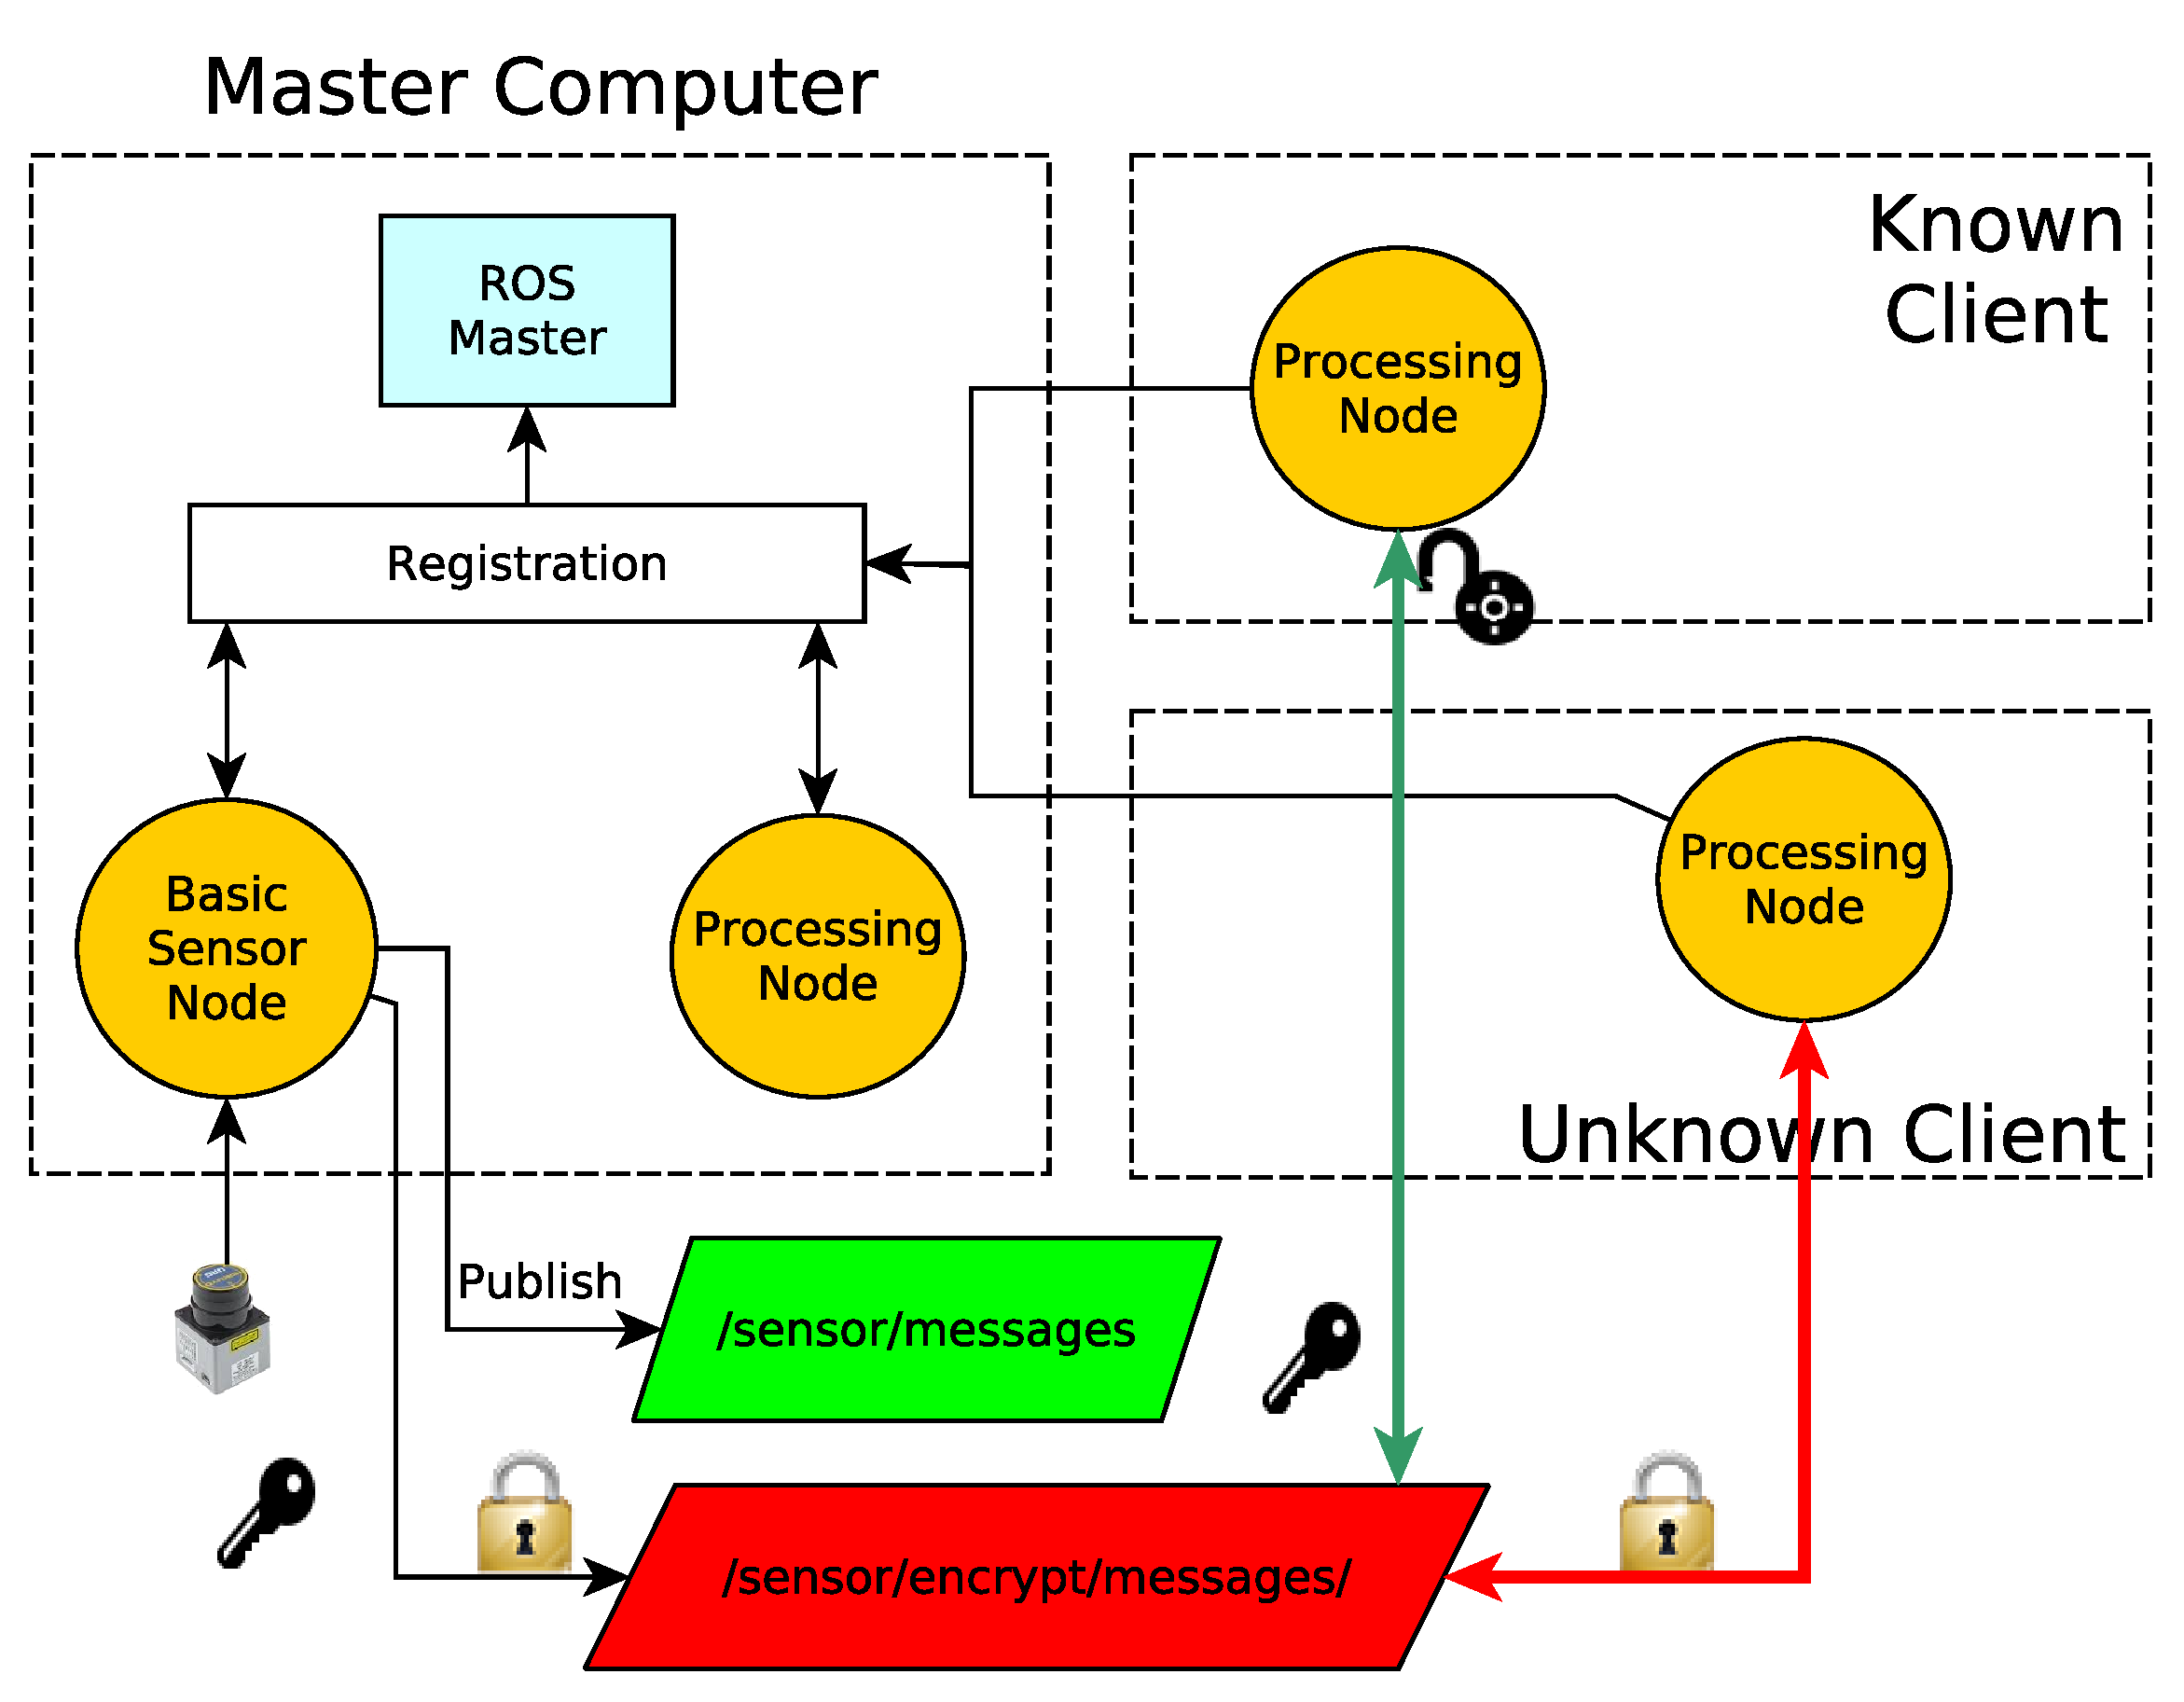
\includegraphics[width=.5\textwidth]{TestBed.pdf}
    \caption{Time spent in each call to encryption/decryption function.}
  \label{fig:TestBed}
\end{figure}







\subsection{Robotic testbed}

We want to evaluate whether ciphering communications would affect the performance of ROS. 
In the second experiment we changed the first computer for a RB1 robot and the XXX switch by a wireless one. This robot was also running ROS Jade.



\section{Experimental Measuments}

Figure \ref{fig:velocidad-maqueta} shows the maximum rate that can be reached both in the laser and the camera visualization according to \texttt{rviz} information.

The same measurements were made in the second environment to see if the use of wireless systems and a real robot would have any influence.

The absolute values of the frame rates is obviously different, as shown in figure \ref{fig:velocidad-robot}. But the interesting part is the relative different when using clear communications or ciphered ones. 

Table \ref{tab:relativas}  compares the relative reduction of speed when using ciphered protocols vs clear ones in both environments as well as the relative increase of CPU usage.

We have addded a funtion to our program in order to measure the time spent in each encrypt and decrypt call. The function is a python method presented as a decorator pattern 
The decorator pattern is used here to extend the functionality of encrypt/decrypt at run-time. 


{
  \footnotesize{
    \begin{Verbatim}[frame=single]
def fn_timer(function):
	  @wraps(function)
	  def function_timer(*args, **kwargs):
	      v_time_0 = time.time()
	      result = function(*args, **kwargs)
	      v_time_1 = time.time()
	      return result
	  return function_timer
    \end{Verbatim}
  }
}


\subsection{Camera}

\subsubsection{Test Messages evaluation}

In this test we have used a modified version of talker/listener tutorial proposed by ROS. 
ROS statistical data shows the simple publish/subscribe example sending 11 string messages ({\em std\_msgs/String}) by second of ``Hello wold'' plus a timestamp with 440 byts of traffic.
In this manner, we want to analyse the behaviour of the system using bigger messages: T1, 262144 bytes; T2,  524288 bytes; and T3, 1048576 bytes 

The measurments of behaviour of ROS traffic presents with simple plain messages {\em delivered\_msgs} 10 of T1 generate . When T2 messages are sent the system runs with 4194368 bytes of traffic and finally when it is working in  T3 messages just send 4194336 bytes and a total of 4 messages. There is no dropped messages by subscribtion.

We want to determine the duration of execution of our talker. We run the Linux {\em time} command to measure the total CPU time consumed by the ROS talker process. 
Firstly we analyzed T1, that presents in a time window of 32.884 seconds a user time of  1.364 seconds and a sys time of 0.044s. It represents a CPU time of 1.408 seconds.
Secondly we analyzed T2, that presents in a time window of 33.749 seconds a user time of  2.508 seconds and a sys time of 0.164s. It represents a CPU time of 2.672 seconds.
Finally we analyzed T3, that presents in a time window of 34.731 seconds a user time of  5.140 seconds and a sys time of 0.120s. It represents a CPU time of 5.260 seconds.

This is totally different when we are working with encrypted text messages of type T1, T2 or T3. Fig~\ref{fig:time_text_CPU} presents the main differences. We have repeated the same experiment, but this time calling an encryption method that encrypts from plain text to DES3. It is possible to see that the encrypt process consumes more CPU than  the plain process.
For instance, T1 type presents running for  34.486 seconds a total of 23.008 of CPU. This means that the total CPU time increases almost 62\%. This is even higher in T2 and T3 types with almost the 98\% of real execution time.
\begin{figure}[h!]
    \centering
    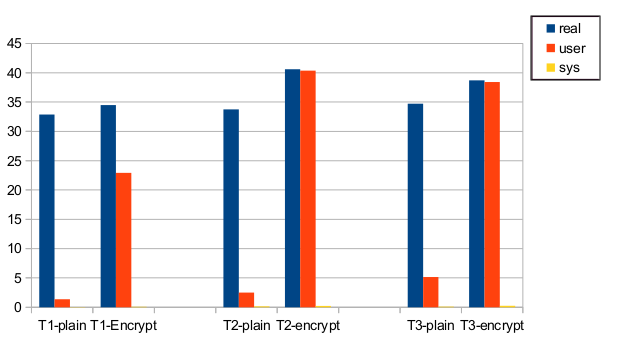
\includegraphics[width=.5\textwidth]{Tiempos_CPU_cifrado_texto.png}
    \caption{Time of CPU spent in a simple talker/listener test.}
  \label{fig:time_text_CPU}
\end{figure}

If we focus in encryption/decryption process we can see the time needed to encryption call presents in 1040 messages 
a minimal time of 0.059246 seconds and a  max time to encrypt the string of  0.683408 seconds with an average of 0.063858 seconds and standard deviation of 0.000388.
This time encreases with T2 and T3 types. T2 type needs 0.123383 seconds in average with standard deviation of 0.000040 seconds and  T3  0.247303 with a standar deviation of 0.000137.
Fig~\ref{fig:text_encryption_time} outlines the behaviour of the talker cyphering data. Left part of the figure presents the box plot of the three types of message. The right part of the element present the number of repetition associated to a time to each encryption process.
\begin{figure*}[ht]
    \centering
    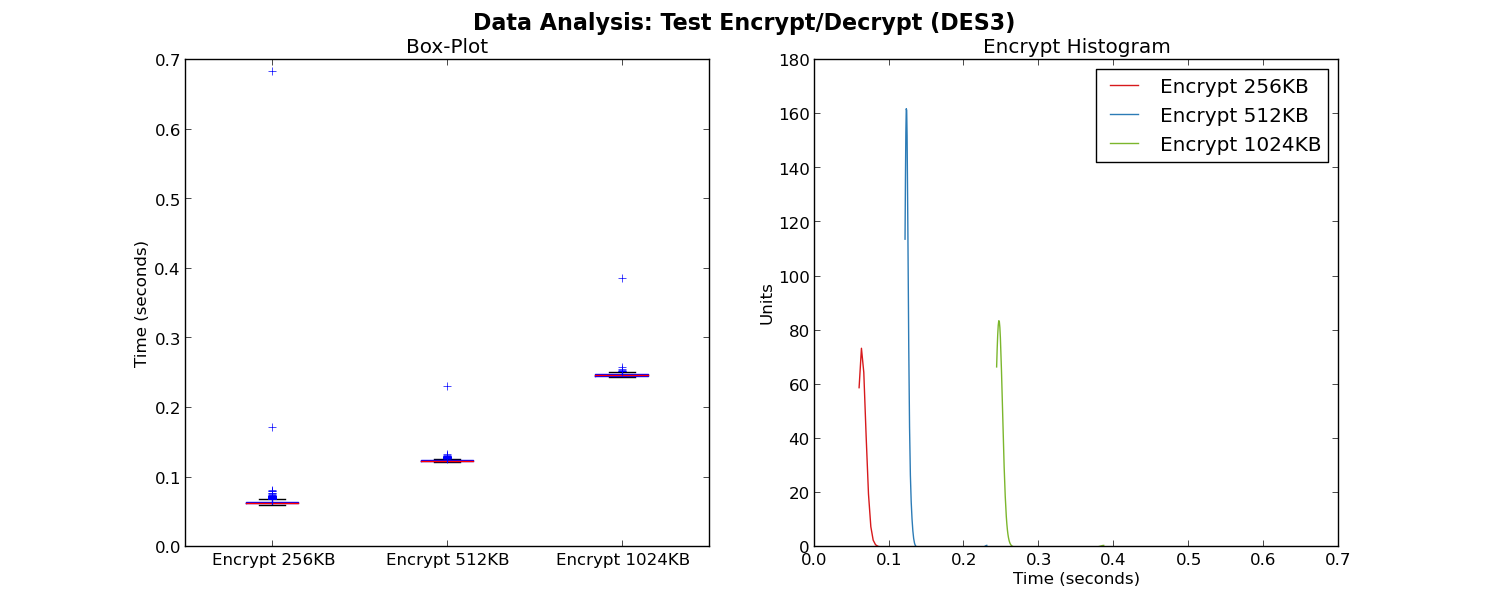
\includegraphics[width=.9\textwidth]{Outline_encryption_text.png}
    \caption{Time spent in each call to encryption/decryption function.}
  \label{fig:text_encryption_time}
\end{figure*}


% raspberry@david-H97M-D3H:~/catkin_ws/src/security_repo/ciphering_project/simple_talker_listener/src$ time python talker3DES.py
% ;;;;;;;;
% ^C
% real    0m34.486s
% user    0m22.924s
% sys    0m0.084s
% raspberry@david-H97M-D3H:~/catkin_ws/src/security_repo/ciphering_project/simple_talker_listener/src$ time python talker3DES.py
% ;;;;;;;;
% ^C
% real    0m40.607s
% user    0m40.368s
% sys    0m0.232s
% raspberry@david-H97M-D3H:~/catkin_ws/src/security_repo/ciphering_project/simple_talker_listener/src$ time python talker3DES.py
% ;;;;;;;;
% ^C
% real    0m38.718s
% user    0m38.416s
% sys    0m0.248s



% where 0m34.731s of execution 
% user    0m5.140s
% sys    0m0.120s
% 
% raspberry@david-H97M-D3H:~/catkin_ws/src/security_repo/ciphering_project/simple_talker_listener/src$ time python talker.py
% ^C
% real    0m33.749s
% user    0m2.508s
% sys    0m0.164s
% 
% raspberry@david-H97M-D3H:~/catkin_ws/src/security_repo/ciphering_project/simple_talker_listener/src$ time python talker.py
% ^C
% real    0m32.884s
% user    0m1.364s
% sys    0m0.044s
% ======================================
% 256
% ======================================
% Cifrado length: 1040.000000
% Cifrado min: 0.059246
% Cifrado max: 0.683408
% Cifrado mean: 0.063858
% Cifrado stdev: 0.000388
% El valor moda de la fase de cifrado fue:
% (array([ 0.06053495]), array([ 3.]))
% ======================================
% 512
% ======================================
% Cifrado length: 309.000000
% Cifrado min: 0.120618
% Cifrado max: 0.229785
% Cifrado mean: 0.123383
% Cifrado stdev: 0.000040
% El valor moda de la fase de cifrado fue:
% (array([ 0.12165689]), array([ 2.]))
% ======================================
% 1024
% ======================================
% Descifrado length: 147.000000
% Descifrado min: 0.242966
% Descifrado max: 0.386008
% Descifrado mean: 0.247303
% Descifrado stdev: 0.000137
% El valor moda de la fase de descifrado fue:
% (array([ 0.24460196]), array([ 2.]))





\subsection{Camera}

\subsubsection{Process evaluation}

We have used a Logitech, Inc. QuickCam Pro 9000 webcam.

There are three nodes involved in our system: usb\_cam, encrypte\_node and decrypted\_node. The first and the sencond run in the master computer, the decrypted one in a separate computer.

There are three topics involved: 

To analyse the behaviour of the system under encrypt/decrypt circumstances we use an intel i7 computer with 16 GM RAM. The ROS master system has 234 process running by default in a Ubuntu 14.04, the client is running 242 process in the same operative system.

In this case we measure the time needed to encrypt or decrypt the ROS message ({\em sensor\_msgs/Image.msg}). We just encrypt or decrypt the field data of {\em uint8[]} that is treated as a string.

This experiment was running for about 18 hours sending in total 971790 frames. The minimal time to encrypt the images was 0.001309 seconds, the max time  0.026909 seconds with a 
mean of  0.010948 seconds and a standard deviation of 0.000004 seconds. The mode value in this phase was 0.010571 seconds wich was reapeated 415 times. 

The minimal time to decrypt the images was 0.001288 seconds, the max time was 0.039130 seconds with a 
mean of  0.008828 seconds and a standard deviation of 0.000003 seconds. The mode value in this phase was 0.008183 seconds wich was reapeated 593 times. 


The figure~\ref{fig:graphicalRepresentation} presents the box-plot of the encryption decryption data analyzed and the histograma. 

\begin{figure}[ht]
    \centering
    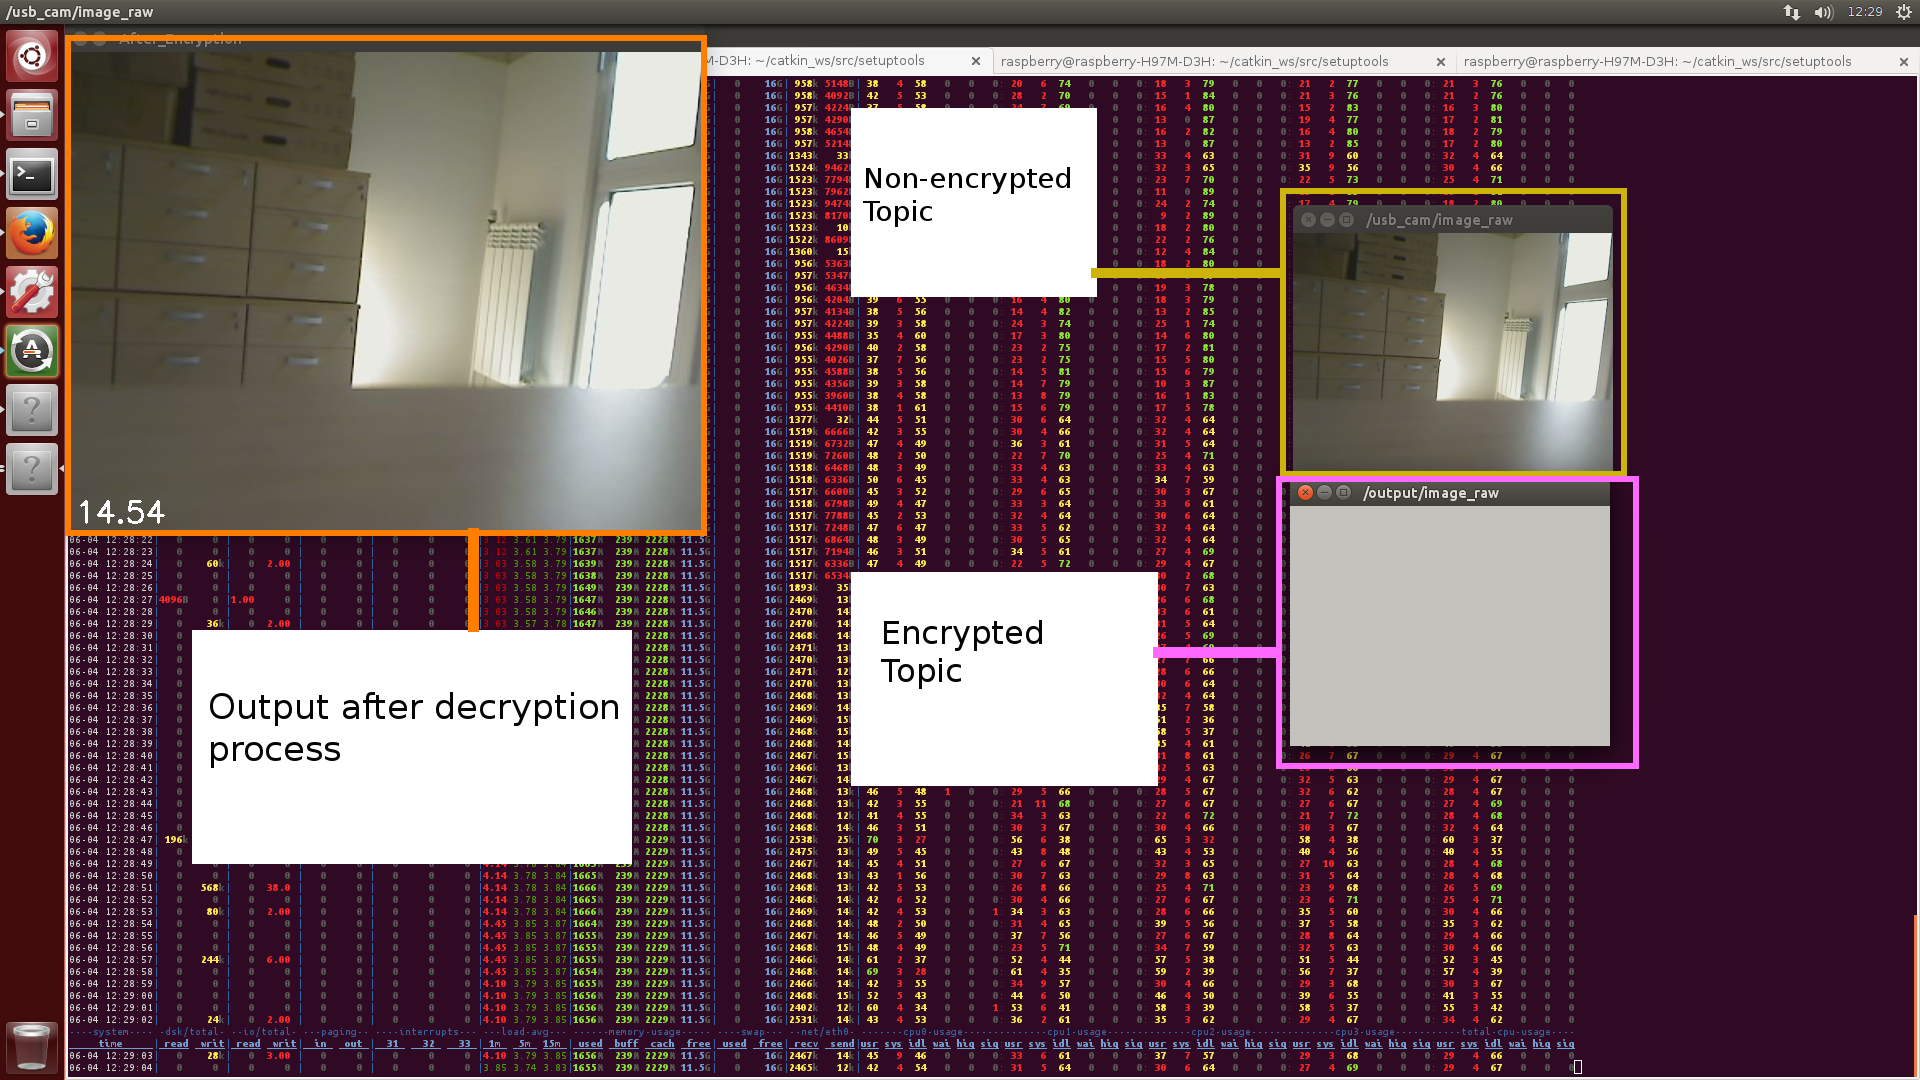
\includegraphics[width=.5\textwidth]{Screenshot.png}
    \caption{Time spent in each call to encryption/decryption function.}
  \label{fig:graphicalRepresentation}
\end{figure}


Our application present the frame rate during the execution in master and client machines. The fps in the encrypter machine is 14.56 and the fps in the decryption machine is 14.54.
We observe that the delay induced by encryption does not reduce the standard frame rate. 




Figure \ref{fig:images_encryption} presents the situation in the client node. We have used the ROS node {\em image\_view} to visualize the images from topics.  There is an non-encrypted topic that we have maintanined in order to validate delays. There is an encrypted topic that is not possible to visualize using the releeased image\_view ROS node. Finally there is a frame that presents the image after decrypt the topic using our own decrypt node. 

\begin{figure*}[ht!]
    \centering
    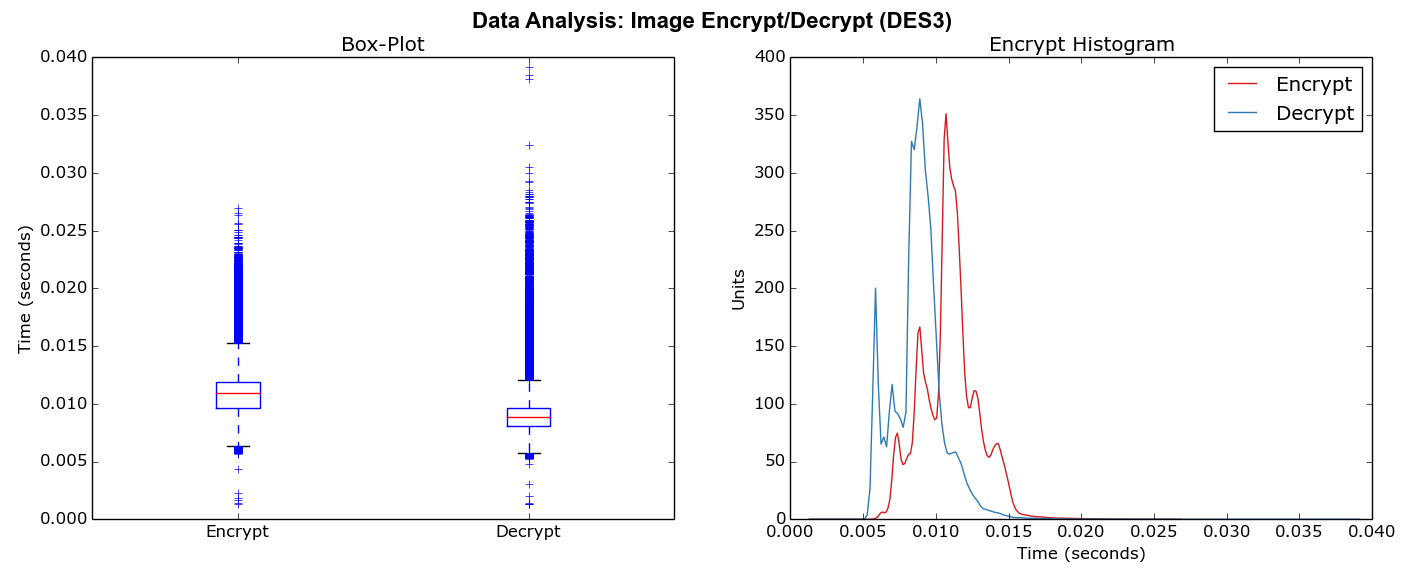
\includegraphics[width=.9\textwidth]{Outline_images_encryption_decrytiontime2.png}
    \caption{Time spent in each call to encryption/decryption function.}
  \label{fig:images_encryption}
\end{figure*}



% Descifrado length: 969295.000000
% Descifrado min: 0.001288
% Descifrado max: 0.039130
% Descifrado mean: 0.008828
% Descifrado stdev: 0.000003
% El valor moda de la fase de descifrado fue:
% (array([ 0.008183]), array([ 593.]))
% At the same time 
% 
% PC descifrador: 242 process (ps -ef | wc -l)
% 
% Cifrador
% [INFO] Encrypter node:  elasped time: 66755.17
% [INFO] Encrypter node:  approx. FPS: 14.56
% 
% 
% 
% Descifrador
% [INFO] Decrypter node: elapsed time: 66659.74
% [INFO] Decrypter node: approx. FPS: 14.54





\section{Conclusion and Futher Work}

We have evaluated the influence of cyphering in the performance of ROS based robotic systems.

As we commented in the introduction, we think that securing communications is just one dimension in  the cybersecurity of Autonomous Systems. If we want to see autonomous systems working in our homes we need to secure the navigation abilities, the interaction mechanisms, etc. 
 
Some works have been sketched in this area, as for instance in \cite{Guiochet2016}.




\section*{Acknowledgment}
The authors would  like to thank the Spanish Ministry of Economy and Competitiveness for the partial support to this work under grant DPI2013-40534-R and to the Spanish National Institue of CyberSecurity (INCIBE) under grand Adenda21 ULE-INCIBE.

\bibliographystyle{plain} 
\bibliography{waf2016}

\end{document}


